\section{Document Editor}
\label{prototype:DocumentEditor}
Documents are my more formal, typed notes. They are designed to be used for more structured note taking such as writing essays, reports or other formal documents. They can also be used for more creative writing such as poetry or short stories. Here are some images from the urrent version of my document editor complete with:
\begin{itemize}
    \item lists
    \item highlighting
    \item automatic code formatting (very helpful for someone making a project about a coded tool :)
    \item quotes
    \item Youtube Embed
    \item Beautiful Maths and chemiacl equations
    \item Collpasible sections
    \item Link
    \item \textbf{and so much more!}
\end{itemize}

\begin{figure}[H]
    \centering
    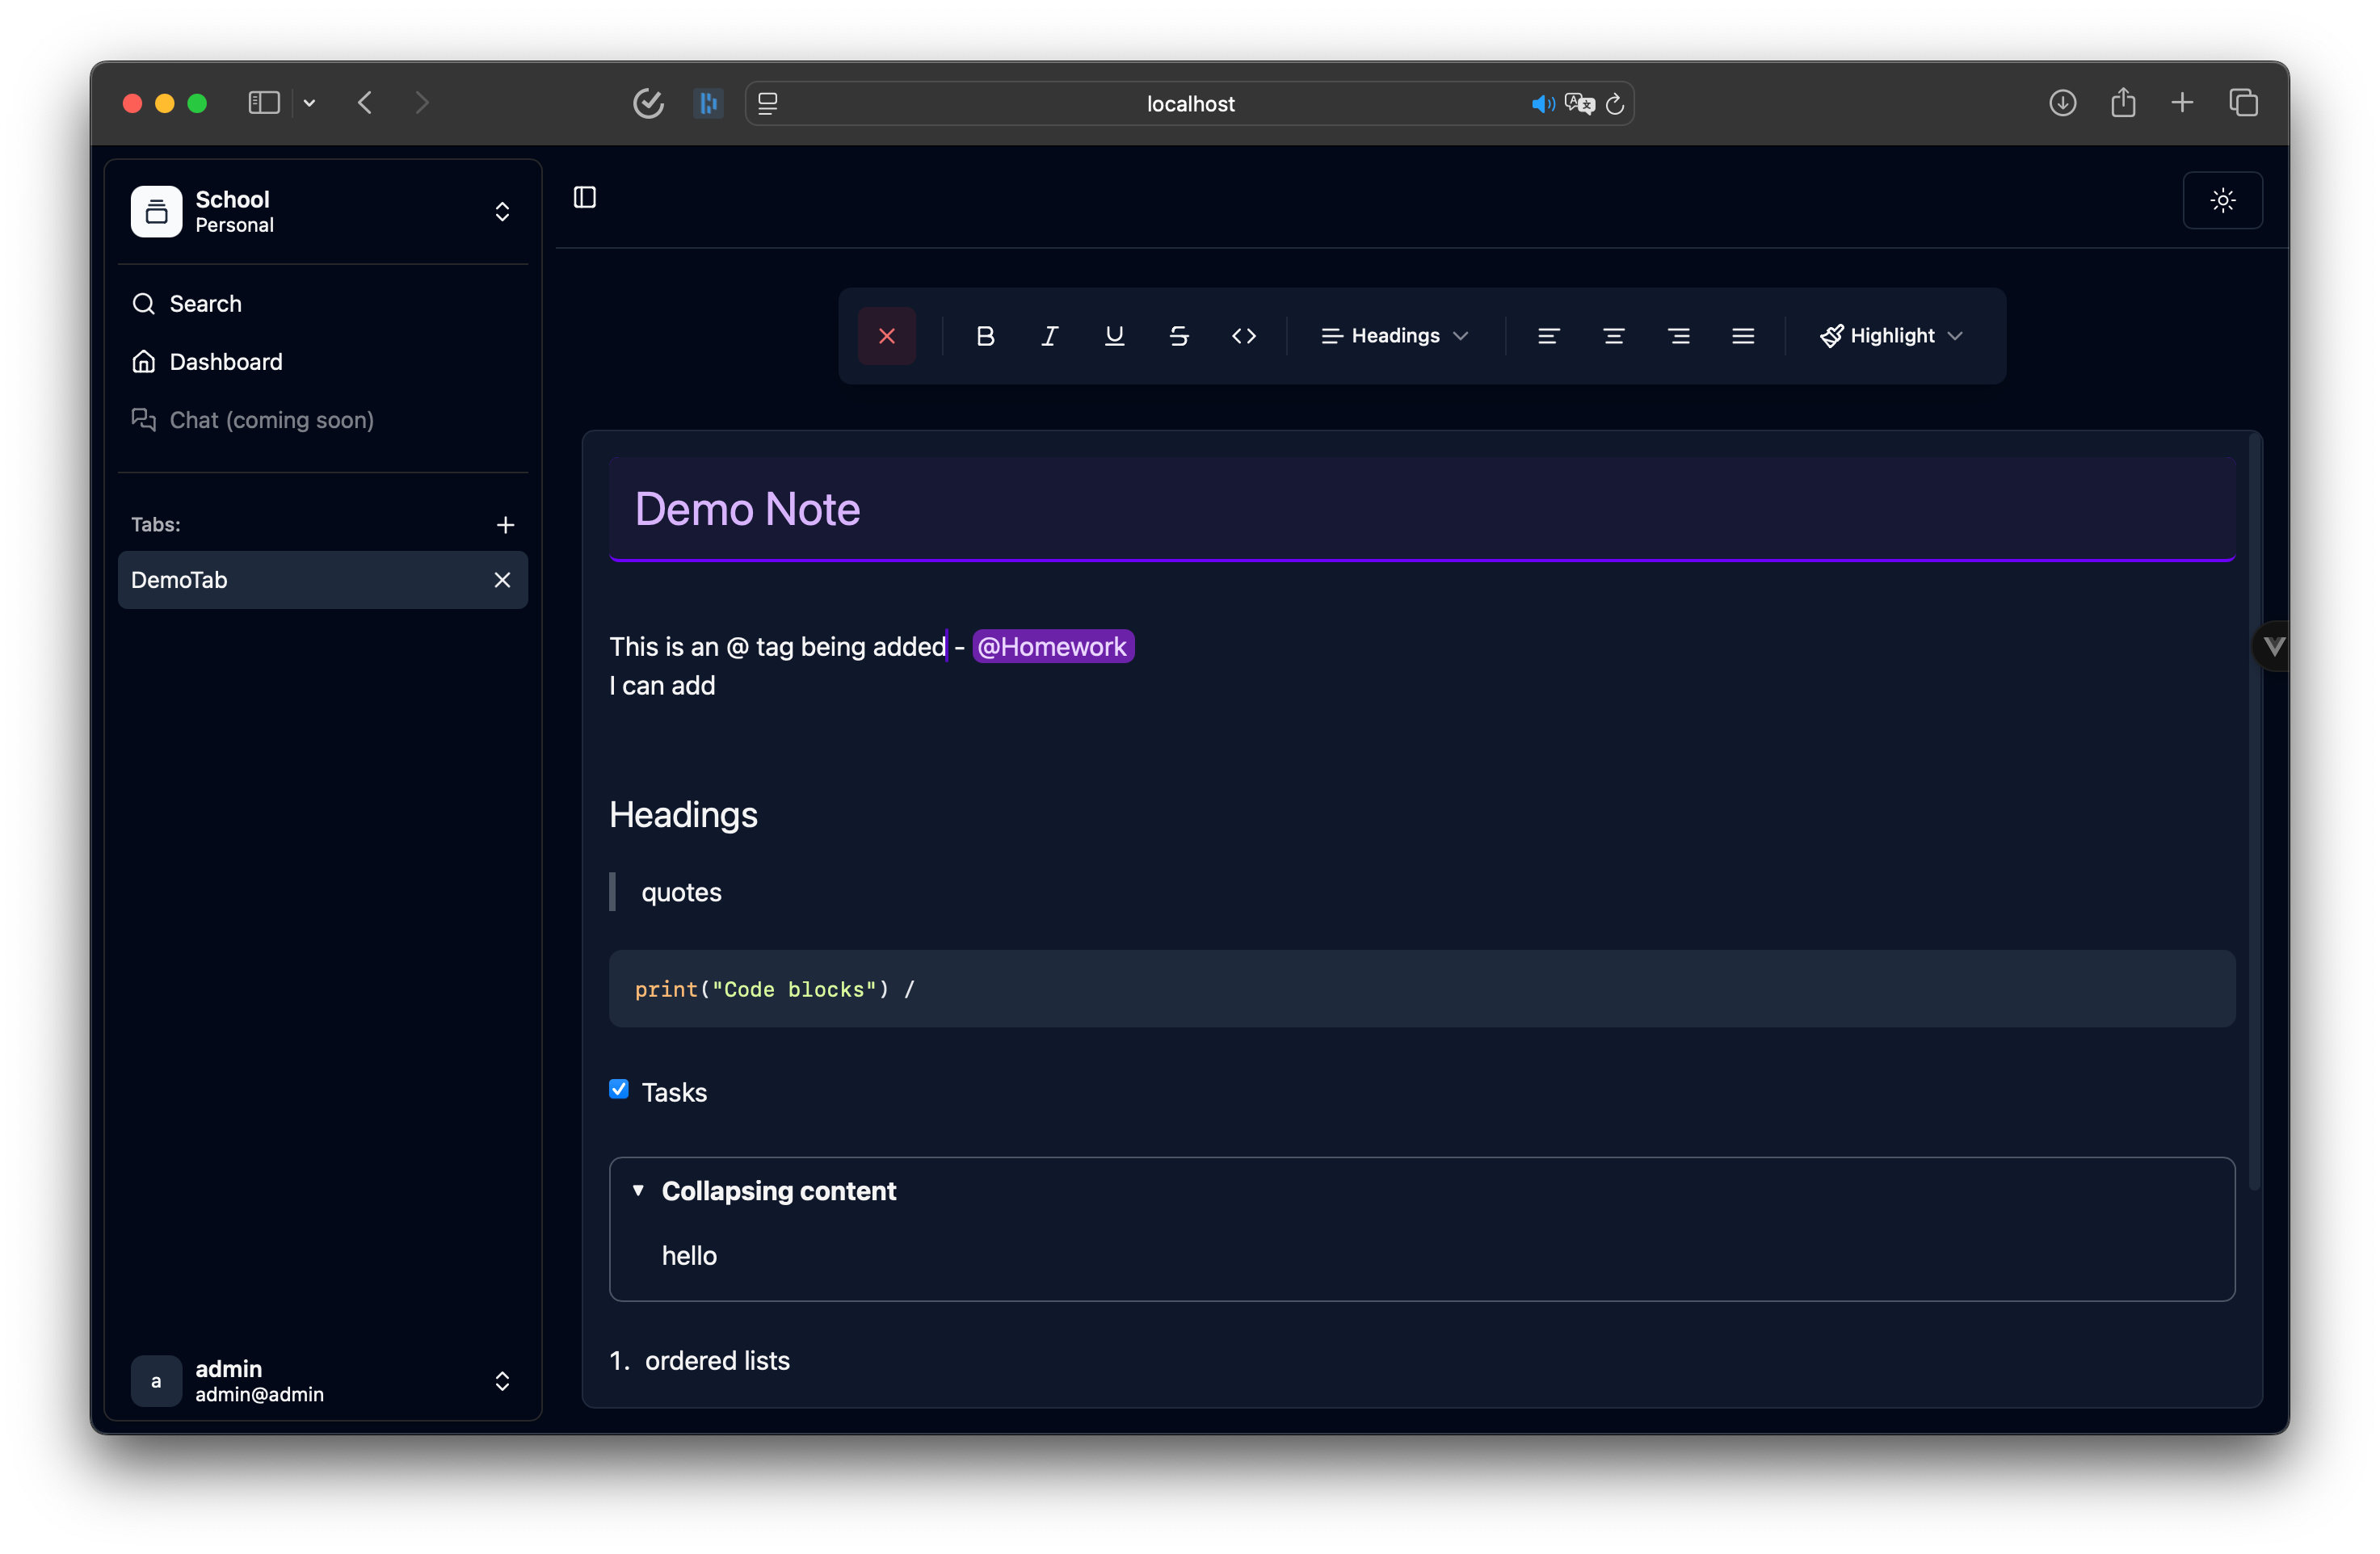
\includegraphics[width=0.8\textwidth]{Prototype/20_DocumentEditor/media/editor1.png}
    \caption{Sample Note}
    \label{artifact:DocumentEditor}
\end{figure}

\begin{figure}[H]
    \centering
    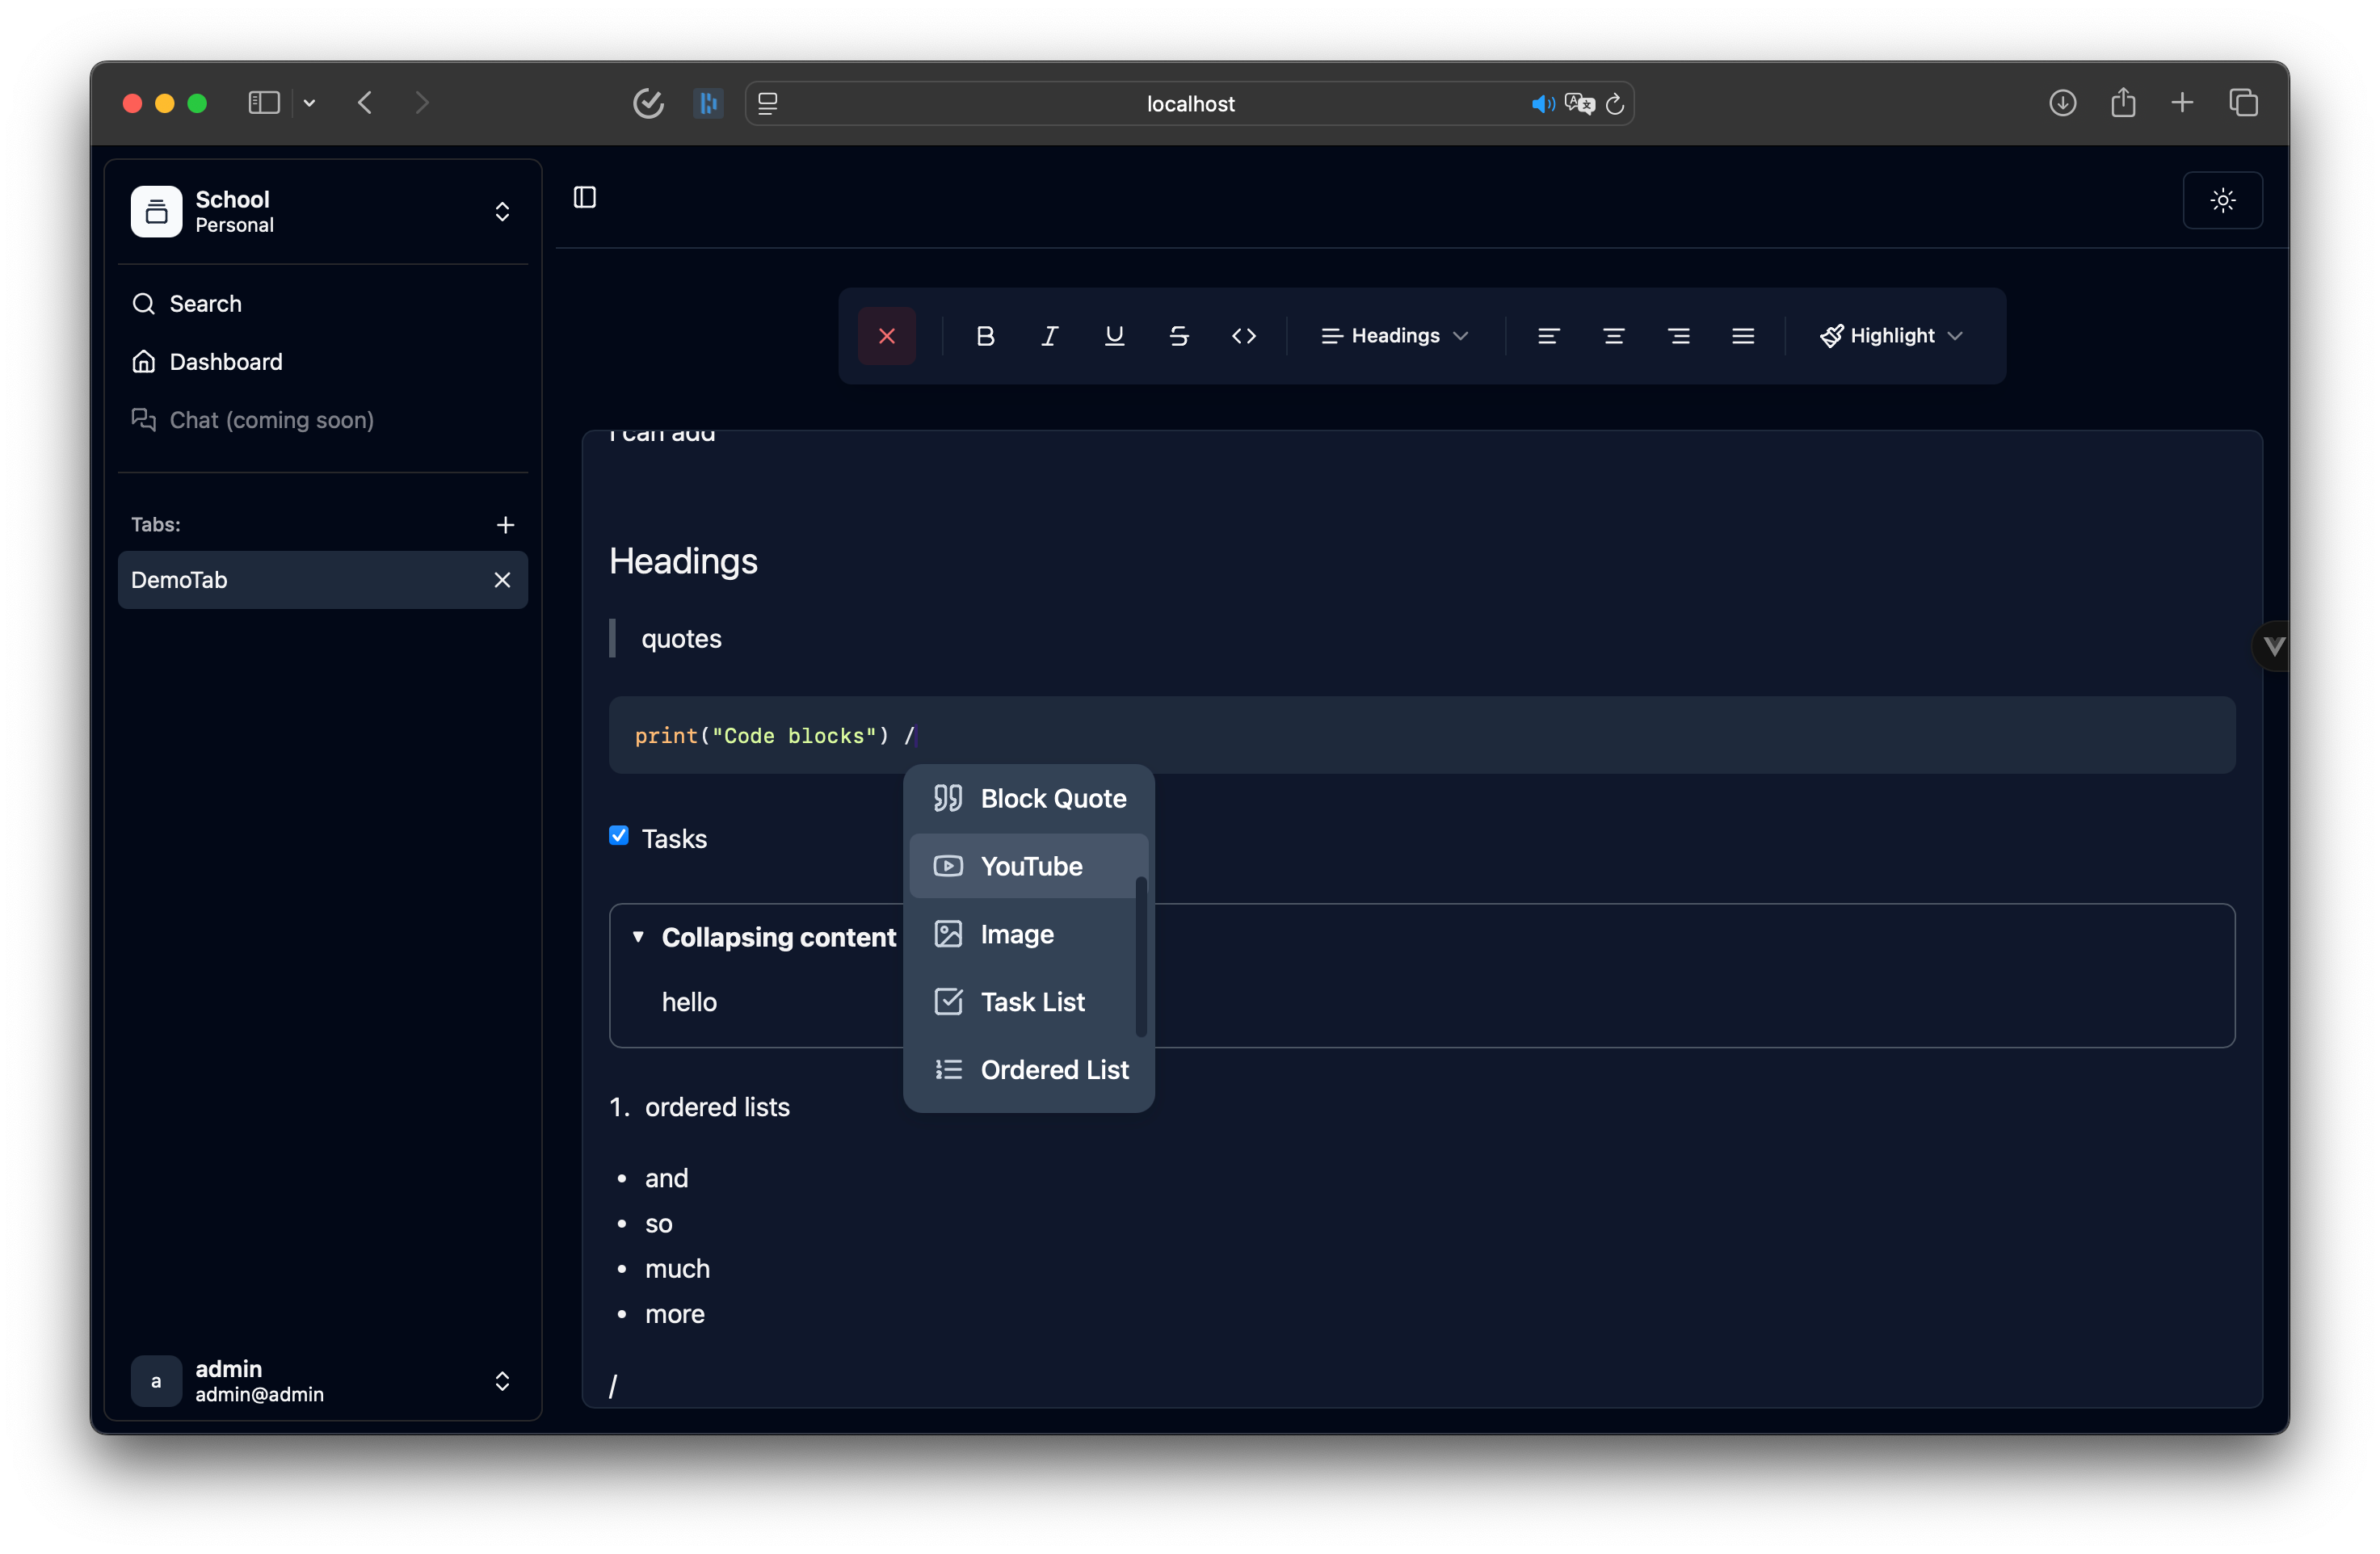
\includegraphics[width=0.8\textwidth]{Prototype/20_DocumentEditor/media/editor2.png}
    \caption{Adding new 'blocks'}
    \label{artifact:DocumentEditor}
\end{figure}